\section{BC01 - Construction et alimentation d'une infrastructure de gestion de données}

% ===
% Infrastructure
% ===

\begin{frame}
    \centering
    \huge
    BC01 - Construction et alimentation d'une infrastructure de gestion de données
\end{frame}

\begin{frame}{Infrastructure conceptualisée}
    \textbf{Architecture générale du système}

    \begin{itemize}
        \item Infrastructure entièrement containerisée via Docker Compose
        \item Architecture orientée Machine Learning Platform
        \item Séparation stockage / traitement / expérimentation
    \end{itemize}

    \vspace{0.4cm}

    \textbf{Composants principaux}

    \begin{itemize}
        \item \textbf{Stockage objet :} MinIO (audio, datasets, artefacts ML)
        \item \textbf{Bases de données :} MongoDB + PostgreSQL
        \item \textbf{Orchestration / ML :} MLflow (tracking expérimental)
        \item \textbf{Traitement distribué :} Apache Spark (cluster master/worker)
    \end{itemize}

    \vspace{0.4cm}

    \textbf{Objectif :} assurer reproductibilité, scalabilité et traçabilité des données
\end{frame}

\begin{frame}{Infrastructure conceptualisée}
    \begin{figure}[h]
        \centering
        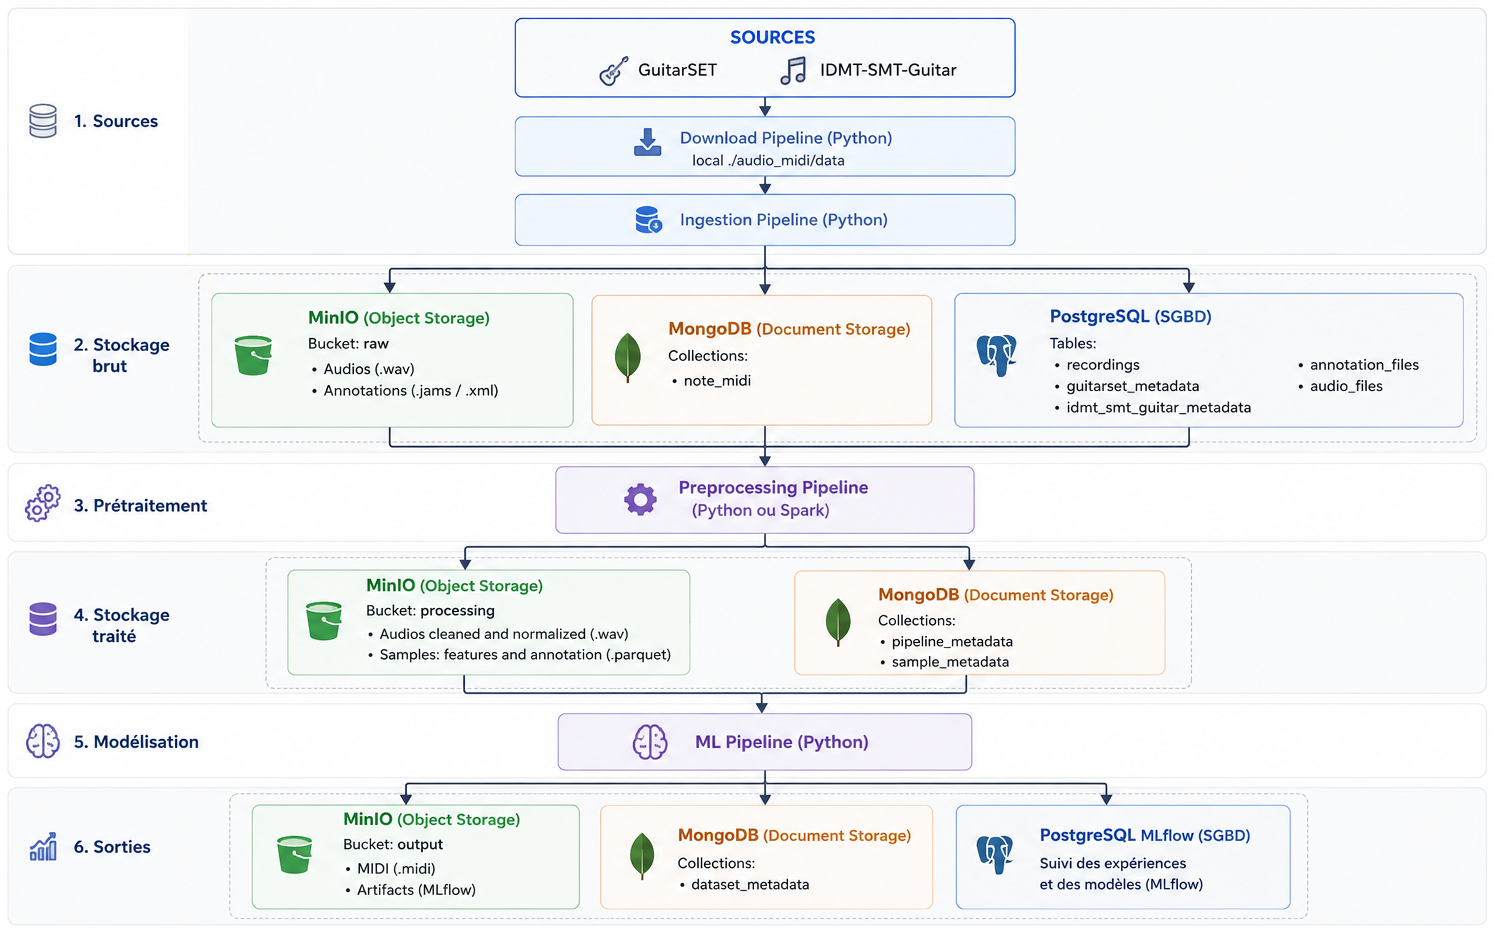
\includegraphics[width=0.7\textwidth]{figures/BC01/architecture_globale.png}
        % \caption{Architecture globale}
        \label{fig:architecture_globale}
    \end{figure}
\end{frame}

% ===
% Collecte
% ===

\begin{frame}{Collecte des données}
    \textbf{Sources de données}

    \begin{itemize}
        \item GuitarSet : enregistrements audio de guitare + annotations MIDI.
        \item IDMT-SMT-Guitar : 4 datasets audio annoté orienté transcription musicale.
    \end{itemize}

    \vspace{0.4cm}

    \textbf{Nature des données collectées}

    \begin{itemize}
        \item Fichiers audio (WAV).
        \item Fichiers d'annotation (JAMS, XML, CSV, TXT).
        \item Métadonnées associées aux fichiers d'annotations.
    \end{itemize}

    \vspace{0.4cm}

    \textbf{Stockage locale}

    \begin{itemize}
        \item Téléchargement locale des archives (ZIP).
        \item Extraction locale des archives.
    \end{itemize}
\end{frame}

% ===
% Ingestion
% ===

\begin{frame}{Ingestion des données}
    \textbf{Pipeline d'ingestion}

    \begin{itemize}
        \item Upload des datasets vers MinIO (bucket \textit{raw})
        \item Extraction des annotations MIDI dans MongoDB (collection \textit{note\_midi})
        \item Extraction des métadonnées dans PostgreSQL
    \end{itemize}

    \vspace{0.4cm}

    \textbf{Sortie du bloc}

    \begin{itemize}
        \item Données prêtes pour analyse exploratoire (Bloc 2)
    \end{itemize}
\end{frame}